\documentclass[skript.tex]{subfiles}

\begin{document}
	\begin{bem}
		Die Dimension einer Mannigfaltigkeit ist wohldefiniert. ---
		Eine nichtleere Teilmenge des $\R^n$ ist genau dann eine
		$n$-dimensionale Mannigfaltigkeit, wenn sie offen ist.
	\end{bem}
	
	\begin{notat}[Lineare Algebra]
		Sei $X$ ein endlich-dimensionaler (reeller) Vektorraum mit innerem Produkt $\skp{\bcdot}{\bcdot}$.
		Das \emph{orthogonale Komplement} $V^{\perp}$ eines Unterraums $V \sbs X$
		ist durch
		\[
			V^{\perp} = \{ x\in X \mid \skp{x}{v}=0 \quad \forall v\in V\}
		\]
		gegeben, und wir haben $V \oplus V^{\perp}=X$.
		Ist $Y$ ein weiterer endlich-dimensionaler Vektorraum
		und $A \colon X \to Y$ eine lineare Abbildung, so setzen wir
		\begin{alignat*}{2}
			\kernel A &= \{x\in X \mid Ax=0\} &&\sbs X, \\
			\image A &= \{Ax \mid x\in X\} &&\sbs Y,
		\end{alignat*}
		und es gilt $\underbrace{\dim\kernel}_{\text{Defekt}} A + \underbrace{\dim\image}_{\text{Rang}} A = \dim X$.
	\end{notat}

	\begin{theorem}
		Für $m,n\in\N$, $m\le n$ und eine nichtleere Menge $M \sbs \R^n$
		sind die folgenden Aussagen äquivalent:
		\begin{enumerate}[(i)]
			\item \emph{(Untermannigfaltigkeit)}\quad
			Für jedes $\xi \in M$ gibt es eine offene Umgebung $\Omega  \sbs \R^n$
			von $\xi$, eine Menge $U \sbs\R^{m}$ und eine Immersion $ \phi\in C^1(U,\R^n)$,
			die $U$ homöomorph auf
			\[
				M\cap\Omega =  \phi(U)
			\]
			abbildet.
			
			\item \begin{minipage}[t]{.55\textwidth}
				\emph{(Gleichungsdefinierte Mannigfaltigkeit)}\quad
				Zu jedem ${\xi \in M}$ gibt es eine offene Umgebung $\Omega \sbs \R^n$ von $\xi$ und eine Abbildung $f \in C^1(\Omega,\R^{n-m})$ mit
				$ \rank \diff f(x)=n-m \:\forall x\in\Omega$ und
				\[
					M \cap \Omega = f^{-1}(\{0_{\R^{n-m}}\}).
				\]
			\end{minipage}
			\hfill
			\begin{minipage}[t][.2\textwidth][b]{.3\textwidth}
				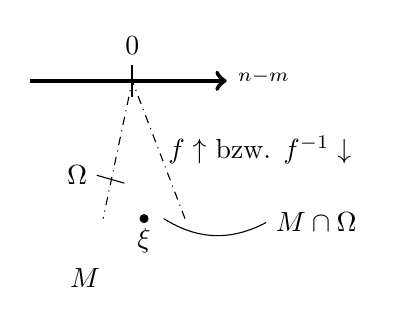
\begin{tikzpicture}
					\saucer{0}{0}{.75};
					\draw[->,ultra thick] (.5,2.5)--(3,2.5) node[right]{$\R^{n-m}$};
					\draw[thick] (1.8,2.3)--(1.8,2.7) node[above]{$0$};
					\draw[dashdotted] (2.47,.75)-- node[right]{$f\uparrow$ bzw. $f^{-1}\downarrow$ } (1.8,2.5)--(1.43,.75);
					
					\node at (1.2,0){$M$};
					\filldraw (1.95,.75) circle[radius=.05] node[below]{$\xi$};
					\draw (1.7,1.2)--(1.35,1.3) node[left]{$\Omega$};
					\draw (3.5,.7) node[right]{$M\cap\Omega$} to[bend left] (2.2,.75);
				\end{tikzpicture}
			\end{minipage}
			
			\item \emph{(Graphendarstellung)}\quad
			Zu jedem $\xi \in M$ gibt es eine offene Umgebung $\Omega \sbs \R^n$ von $\xi$,
			eine offene Menge $U \sbs\R^{m}$ und ein $g \in C^1(U,\R^{n-m})$ mit
			\[
				M\cap\Omega = \Pi(\graph g),
			\]
			wobei $\Pi \in \mathrm{GL}(n)$ eine Permutationsmatrix ist.
		\end{enumerate}
	\end{theorem}
	Eine Permutationsmatrix $\Pi$ ist durch einen Zykel\footnote{zyklische Permutation, siehe Lineare Algebra I} $\sigma\in\mf{S}_{n}$
	eindeutig charakterisiert, und es gilt
	$\Pi e_{j}=e_{\sigma(j)}$ für $j=1,\dotsc, n$.
	\begin{proof}
		\emph{„(i)$\implies$(ii)“}\quad Wir konstruieren eine Funktion $f$ mithilfe des Umkehrsatzes.\\
		Sei also $M$ eine $m$-dimensionale Untermannigfaltigkeit des $\R^n$ wie in \emph{(i)} und \\
		$\eta = \phi^{-1}(\xi) \in U$. Da $\phi$ eine Immersion ist, besitzt $\diff \phi(\eta)$ einen vollen Rang und die Spalten von $\diff\phi$ spannen einen linearen Unterraum $T$ auf.
		\begin{center}
			\fbox{
				\begin{minipage}{.4\textwidth}
					\vspace{.4\textwidth}
					Grafik folgt in Kürze.
					\vspace{.4\textwidth}
				\end{minipage}
			}
		\end{center}
		Mit $P_T$ bezeichnen wir die orthogonale Projektion $\R^n \to T\sbs\R^n$. Weiterhin setzen wir $\phi_T \ceq P_T \circ \phi \colon U \to T \sbs \R^n$. Insbesondere gilt $\rank \diff\phi_T = m$, denn
		\[
			\diff\phi_T = \diff(P_T \circ \phi) =\footnotemark \underbrace{((\diff P_T)\circ\phi)}_{= P_T} \diff\phi.
		\]
		\footnotetext{
			$A = P_T, v\in\R^n$
			\[
				\frac{A(x+\tau v)-A(x)}{\tau} = Av \implies \diff A = A
			\]
		}
		Entsprechend ist
		\[
			\diff\phi_T(\R^n) = P_T\underbrace{\diff\phi(\R^n)}_{= T}=T.
		\]
	\end{proof}
\end{document}